% !TeX program = xelatex
\documentclass[a4paper,10pt]{article}

% ============================================================================
% សន្លឹកកិច្ចការសិស្សបំពេញចន្លោះ ស-ខ្មៅ និងប្លង់ក្ដារខៀន/ចម្លើយគ្រូ (គ្មាន LCD / គ្មានកន្ត្រៃ)
% មេរៀនទី១ (១-៣)៖ សញ្ញាណ លំដាប់ និងចំនួនគត់គូនិងសេស — ត្រូវគ្នា ១០០% នឹង LS_Plan_WN11.tex
% ============================================================================
\usepackage[a4paper, left=1.0cm, right=1.0cm, top=0.75cm, bottom=1.00cm, footskip=0.52cm]{geometry}
\usepackage{amsmath}
\usepackage{unicode-math}
\usepackage{fontspec}
\usepackage{array, colortbl}
\usepackage[table]{xcolor}
\usepackage{enumitem}
\usepackage{pifont}
\usepackage{fancyhdr}
\usepackage{lastpage}
\usepackage{tikz}
\usepackage[most]{tcolorbox}
\usetikzlibrary{calc, arrows.meta, decorations.pathreplacing, positioning, babel}

\makeatletter
\let\@expl@@@mark@update@singlecol@structures@@\relax
\makeatother

\providecommand{\NGSFindFonts}{%
  \IfFileExists{C:/Windows/Fonts/cambria.ttc}{%
    \def\NGSSysPath{C:/Windows/Fonts/}%
    \def\NGSUserPath{C:/Users/KIT/AppData/Local/Microsoft/Windows/Fonts/}%
  }{%
    \IfFileExists{./fonts/KhmerOSsiemreap.ttf}{\def\NGSSysPath{./fonts/}\def\NGSUserPath{./fonts/}}{%
    \IfFileExists{../fonts/KhmerOSsiemreap.ttf}{\def\NGSSysPath{../fonts/}\def\NGSUserPath{../fonts/}}{%
    \IfFileExists{../../fonts/KhmerOSsiemreap.ttf}{\def\NGSSysPath{../../fonts/}\def\NGSUserPath{../../fonts/}}{%
    \IfFileExists{../../../fonts/KhmerOSsiemreap.ttf}{\def\NGSSysPath{../../../fonts/}\def\NGSUserPath{../../../fonts/}}{%
    \IfFileExists{../../../../fonts/KhmerOSsiemreap.ttf}{\def\NGSSysPath{../../../../fonts/}\def\NGSUserPath{../../../../fonts/}}{%
    \IfFileExists{../../../../../fonts/KhmerOSsiemreap.ttf}{\def\NGSSysPath{../../../../../fonts/}\def\NGSUserPath{../../../../../fonts/}}{%
    \IfFileExists{../../../../../../fonts/KhmerOSsiemreap.ttf}{\def\NGSSysPath{../../../../../../fonts/}\def\NGSUserPath{../../../../../../fonts/}}{%
      \def\NGSSysPath{../../../../../../../fonts/}\def\NGSUserPath{../../../../../../../fonts/}%
    }}}}}}}%
  }%
}
\NGSFindFonts

\setmathfont[Path={\NGSSysPath}, FontIndex=1, Scale=1.02]{cambria.ttc}
\defaultfontfeatures{Ligatures=TeX}

\setmainfont[
  Path={\NGSUserPath}, Extension=.ttf, Script=Khmer,
  BoldFont={KhmerOSsiemreap}, BoldFeatures={FakeBold=1.8},
  ItalicFont={KhmerOSsiemreap}, ItalicFeatures={FakeSlant=0.25},
  BoldItalicFont={KhmerOSsiemreap}, BoldItalicFeatures={FakeBold=1.8, FakeSlant=0.25}
]{KhmerOSsiemreap}

\newfontfamily\muol[Path={\NGSUserPath}, Extension=.ttf, Script=Khmer]{KhmerOSmuollight}
\newfontfamily\TimesEn[Path={\NGSSysPath}, Extension=.ttf, BoldFont={timesbd}, ItalicFont={timesi}, BoldItalicFont={timesbi}]{times}
\newfontfamily\CalibriFont[Path={\NGSSysPath}, Extension=.ttf]{calibri}

\XeTeXlinebreaklocale "km"
\XeTeXlinebreakskip = 0pt plus 1pt minus 0.1pt

\definecolor{panelgray}{gray}{0.94}
\definecolor{headgray}{gray}{0.85}

\pagestyle{fancy}
\fancyhf{}
\renewcommand{\headrulewidth}{0pt}
\fancyfoot[L]{\fontsize{7.4pt}{9.5pt}\selectfont អនុវិទ្យាល័យព្រះក្រសាំង \en{|} គ្រូ៖ ហុក ប៊ុនថែន \en{|} មេរៀនទី១ (១--៣) សញ្ញាណ លំដាប់ និងគូសេស \en{|} ថ្ងៃអង្គារ ទី៣ ខែវិច្ឆិកា ឆ្នាំ២០២៦}
\fancyfoot[R]{\fontsize{7.8pt}{10pt}\selectfont ទំព័រ \en{\thepage\ / \pageref{LastPage}}}

\setlength{\parindent}{0pt}
\setlength{\parskip}{0pt}
\setlength{\tabcolsep}{4pt}

\newcommand{\en}[1]{{\TimesEn #1}}
\newcommand{\enbf}[1]{{\TimesEn\bfseries #1}}
\newcommand{\cnum}[1]{\mbox{\fontsize{10pt}{12pt}\selectfont\ding{\numexpr181+#1\relax}}}
\newcommand{\chkbox}{\tikz[baseline=-0.15ex]\draw[black, line width=0.85pt, fill=white] (0,0) rectangle (0.24cm,0.24cm);}
\newcommand{\ansbox}[1][1.75cm]{\,\tikz[baseline=-0.65ex]\draw[black, line width=0.65pt, fill=white] (0,0) rectangle (#1, 0.42cm);\,}
\newcommand{\dotline}[1][2.2cm]{\makebox[#1]{\dotfill}}

\newcommand{\pagebanner}[2]{%
  \begin{tcolorbox}[
    enhanced, sharp corners, colback=headgray, colframe=black,
    boxrule=1.05pt, boxsep=1pt, top=2.5pt, bottom=2.5pt, left=6pt, right=6pt,
    after skip=3.5pt
  ]
    {\muol\fontsize{9.0pt}{13.2pt}\selectfont #1}\hfill{\fontsize{8.0pt}{11.2pt}\selectfont\textbf{#2}}
  \end{tcolorbox}%
}

\newcommand{\secstrip}[2]{%
  \vspace{3pt}%
  \begin{tcolorbox}[
    enhanced, sharp corners, colback=panelgray, colframe=black,
    boxrule=0.8pt, boxsep=0.8pt, top=2pt, bottom=2pt, left=5pt, right=5pt,
    after skip=3pt
  ]
    {\muol\fontsize{8.5pt}{12.2pt}\selectfont #1}\hfill{\fontsize{7.8pt}{10.8pt}\selectfont\textit{#2}}
  \end{tcolorbox}%
}

\begin{document}
\fontsize{9.5pt}{14.5pt}\selectfont

% ============================================================================
% ទំព័រទី ១៖ សន្លឹកកិច្ចការសិស្ស (ផ្នែកមុខ៖ E1 -> E2 -> E3)
% ============================================================================
\pagebanner{សន្លឹកកិច្ចការសិស្ស \enbf{(}១\enbf{.}១\enbf{--}១\enbf{.}៣ សញ្ញាណ លំដាប់ និងគូសេស\enbf{)} \enbf{--} ផ្នែកមុខ}{ថ្នាក់ទី៧ \en{|} សៀវភៅគោល ទំ.១--៣}

\begin{tcolorbox}[
  enhanced, sharp corners, colback=white, colframe=black,
  boxrule=0.8pt, boxsep=1.5pt, top=3.5pt, bottom=3.5pt, left=5pt, right=5pt,
  after skip=4pt
]
  \fontsize{9.0pt}{13.0pt}\selectfont
  \textbf{ឈ្មោះសិស្ស៖} \dotline[4.3cm] \quad
  \textbf{សមាជិកក្រុម៖} \dotline[4.3cm] \quad
  \textbf{ថ្នាក់ទី៖} ៧\dotline[0.9cm] \quad
  \textbf{ក្រុមទី៖} \dotline[1.0cm]
\end{tcolorbox}

% --- E1 Engage ---
\secstrip{ផ្នែកទី ១ \enbf{(E1 - Engage)} ៖ បេសកកម្មអន្ទាក់លេខសូន្យ ($0$) និងស្លាកលេខផ្ទះគូ}{រយៈពេល ៣ នាទី (គូស \ding{51} ក្នុង \chkbox)}

\begin{tcolorbox}[
  enhanced, sharp corners, colback=white, colframe=black,
  boxrule=0.8pt, boxsep=2pt, top=4pt, bottom=4pt, left=6pt, right=6pt
]
  សិស្សពីរនាក់ជជែកគ្នាអំពីលេខសូន្យ ($0$) និងលេខផ្ទះគូ $n$ ដែលផ្ទៀងផ្ទាត់ $72 < n \le 90$ ៖\\[3pt]
  $\bullet$ \textbf{តើសិស្សរូបណាពន្យល់បានត្រឹមត្រូវ?} \quad
  \chkbox\ \textbf{សិស្ស ក៖} $0$ ជាគត់ធម្មជាតិ (មិនគូ) និងយកទាំង $72$ \quad
  \chkbox\ \textbf{សិស្ស ខ៖} $0$ ជាគត់គូ (មិនធម្មជាតិ) និងយកពី $74$ ដល់ $90$\\[3pt]
  $\bullet$ \textbf{ការស្មានបឋម៖} $0 \div 2 =$ \dotline[1.6cm] ហើយសញ្ញា $<$ ត្រង់ $72 < n$ មានន័យថា $n$ \dotline[3.4cm] នឹង $72$ ។
\end{tcolorbox}

\vfill

% --- E2 Explore ---
\secstrip{ផ្នែកទី ២ \enbf{(E2 - Explore)} ៖ សញ្ញាណ លំដាប់លើបន្ទាត់ចំនួន និងភាពគូ-សេស (ទំ.១--៣)}{រយៈពេល ១១ នាទី}

\textbf{សកម្មភាព ១ (\en{E2-A} — ៦ នាទី)៖ សញ្ញាណចំនួនគត់ និងលំហាត់គំរូ ១ លើបន្ទាត់ចំនួន (ទំ.១--២)}

\begin{tcolorbox}[
  enhanced, sharp corners, colback=white, colframe=black,
  boxrule=0.8pt, boxsep=2.5pt, top=4.5pt, bottom=4.5pt, left=6pt, right=6pt
]
  $\bullet$ ប្រព័ន្ធរបាប់ហ៊ិនឌូអារ៉ាប់មាន ១០ លេខគឺ $0, 1, 2, 3, 4, 5, 6, 7, 8, 9$ ។ «មួយពាន់ប្រាំបួនរយហាសិបបី» តាងដោយលេខ៖ \ansbox[2.2cm]\\[3.5pt]
  $\bullet$ ចំនួន $0, 1, 2, 3, 4, \dots$ ហៅថា \dotline[2.8cm] ឯចំនួនគត់ដែលគ្មាន $0$ ($1, 2, 3, 4, \dots$) ហៅថា \dotline[3.4cm] ។\\[3.5pt]
  $\bullet$ ចំនួនគត់ធំបន្ទាប់ពី $10$ គឺ \dotline[1.3cm] ហើយចំនួនគត់ធំបន្ទាប់ពី $999$ គឺ \dotline[1.6cm] (ចំនួនគត់មានច្រើនរាប់មិនអស់) ។\\[3.5pt]
  $\bullet$ \textbf{លំហាត់គំរូ ១ (ទំ.២)៖} គូសរង្វង់ស ($\circ$) លើចុងដែនមិនយក និងចំណុចខ្មៅ ($\bullet$) តាងចំនួនគត់ \textbf{«ធំជាង $4$ និងតូចជាង $11$»} ៖\\[4pt]
  \begin{center}
  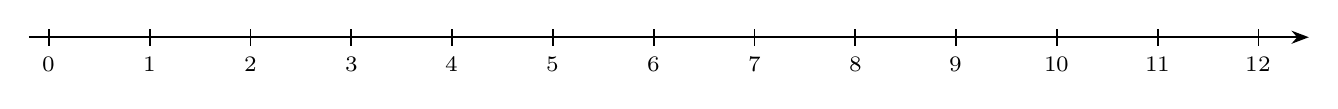
\begin{tikzpicture}[x=1.28cm, y=1cm, every node/.style={font=\footnotesize, text=black}]
    \draw[-{Stealth[length=2.2mm]}, black, line width=0.85pt] (-0.2,0) -- (12.5,0);
    \foreach \i in {0,1,2,3,4,5,6,7,8,9,10,11,12} {
      \draw[black, line width=0.65pt] (\i,-0.11) -- (\i,0.11);
      \node at (\i,-0.34) {$\i$};
    }
  \end{tikzpicture}
  \end{center}
  \vspace{-1pt}
  ដូចនេះ ចំនួនគត់ធំជាង $4$ (នៅខាងស្ដាំ $4$) និងតូចជាង $11$ (នៅខាងឆ្វេង $11$) គឺ ៖ \dotline[7.2cm] ។
\end{tcolorbox}

\vspace{4pt}
\textbf{សកម្មភាព ២ (\en{E2-B} — ៥ នាទី)៖ ចំនួនគត់គូ ចំនួនគត់សេស និងលំហាត់គំរូទំ.៣}

\begin{tcolorbox}[
  enhanced, sharp corners, colback=white, colframe=black,
  boxrule=0.8pt, boxsep=2.5pt, top=4.5pt, bottom=4.5pt, left=6pt, right=6pt
]
  $\bullet$ \textbf{ចំនួនគត់គូ} ជាគ្រប់ចំនួនគត់ដែលចែកដាច់នឹង \dotline[1.2cm] ($0, 2, 4, 6, 8, \dots$); \textbf{ចំនួនគត់សេស} ចែកមិនដាច់នឹង $2$ ($1, 3, 5, 7, \dots$) ។\\[3.5pt]
  $\bullet$ \textbf{លំហាត់គំរូ (ទំ.៣)៖} ចូររកគ្រប់ចំនួនគត់គូនៅចន្លោះ $20$ និង $43$ (កត់សម្គាល់៖ «នៅចន្លោះ» មិនយក $20$ ទេ!) ៖\\[4pt]
  \hspace*{0.3cm}ចម្លើយ ៖ $22, \ 24,$ \dotline[14.8cm] ។
\end{tcolorbox}

\vfill

% --- E3 Explain ---
\secstrip{ផ្នែកទី ៣ \enbf{(E3 - Explain)} ៖ សង្ខេបវិធានគោល និងធនាគារហេតុផល \enbf{B\&W}}{រយៈពេល ៦ នាទី}

\begin{tcolorbox}[
  enhanced, sharp corners, colback=white, colframe=black,
  boxrule=0.85pt, boxsep=2.5pt, top=4pt, bottom=4pt, left=6pt, right=6pt
]
  ១) ចំនួនគត់តូចបំផុតគឺ \dotline[1.1cm] ឯចំនួនគត់ធម្មជាតិតូចបំផុតគឺ \dotline[1.1cm] \quad
  ២) លើបន្ទាត់ចំនួន ចំនួននៅខាងស្ដាំ \dotline[1.6cm] ចំនួននៅខាងឆ្វេង\\[3.5pt]
  ៣) ចំនួនគត់គូបញ្ចប់ដោយលេខ \dotline[3.2cm] ឯចំនួនគត់សេសបញ្ចប់ដោយលេខ \dotline[3.2cm]\\[4pt]
  \tikz\draw[black, dashed, line width=0.5pt] (0,0) -- (18.4cm,0);\\[3.5pt]
  \fontsize{8.8pt}{13.0pt}\selectfont
  \textbf{ធនាគារហេតុផល (\en{Warrant Bank})៖} \quad
  \cnum{1} \textbf{លេខ $0$៖} ជាចំនួនគត់ ប៉ុន្តែមិនមែនជាចំនួនគត់ធម្មជាតិទេ \quad
  \cnum{2} \textbf{បន្ទាត់ចំនួន៖} ខាងស្ដាំ $>$ ខាងឆ្វេង\\
  \cnum{3} \textbf{ចុងដែន៖} សញ្ញា $<, >$ ឬ «នៅចន្លោះ» ($\circ$ មិនយកចុងដែន); សញ្ញា $\le, \ge$ ($\bullet$ យកចុងដែន) \quad
  \cnum{4} \textbf{គូ-សេស៖} ចែកដាច់នឹង $2 \iff$ គូ ($0,2,4,6,8$)
\end{tcolorbox}

% ============================================================================
% ទំព័រទី ២៖ សន្លឹកកិច្ចការសិស្ស (ផ្នែកខាងខ្នង៖ E4 -> E5 -> កិច្ចការផ្ទះ)
% ============================================================================
\clearpage
\pagebanner{សន្លឹកកិច្ចការសិស្ស \enbf{(}១\enbf{.}១\enbf{--}១\enbf{.}៣ សញ្ញាណ លំដាប់ និងគូសេស\enbf{)} \enbf{--} ផ្នែកខាងខ្នង}{ថ្នាក់ទី៧ \en{|} សៀវភៅគោល ទំ.២--៣ និង ទំ.១៤}

% --- E4 Elaborate ---
\secstrip{ផ្នែកទី ៤ \enbf{(E4 - Elaborate)} ៖ លំហាត់គំរូ ២ — រៀបឆ្លាស់លេខ $3, 4, 5$ រកចំនួនធំបំផុតនិងតូចបំផុត (ទំ.២)}{រយៈពេល ១០ នាទី}

\begin{tcolorbox}[
  enhanced, sharp corners, colback=white, colframe=black,
  boxrule=0.8pt, boxsep=2.5pt, top=4.5pt, bottom=4.5pt, left=6pt, right=6pt
]
  បើគេរៀបឆ្លាស់លេខ $3, 4, 5$ តើគេអាចបង្កើតចំនួន ៣ ខ្ទង់ផ្សេងគ្នាបានប៉ុន្មាន? តើចំនួនធំបំផុតស្មើនឹងប៉ុន្មាន? ចំនួនតូចបំផុតស្មើនឹងប៉ុន្មាន?\\[4pt]
  \begin{center}
  {\renewcommand{\arraystretch}{1.28}
  \begin{tabular}{|p{5.5cm}|p{5.5cm}|p{5.5cm}|}
    \hline
    \cellcolor{panelgray}\centering\textbf{ចាក់សោខ្ទង់រយលេខ $3$} &
    \cellcolor{panelgray}\centering\textbf{ចាក់សោខ្ទង់រយលេខ $4$} &
    \cellcolor{panelgray}\centering\textbf{ចាក់សោខ្ទង់រយលេខ $5$} \tabularnewline \hline
    \centering $345$ \quad និង \quad \dotline[1.6cm] &
    \centering $435$ \quad និង \quad \dotline[1.6cm] &
    \centering $534$ \quad និង \quad \dotline[1.6cm] \tabularnewline \hline
  \end{tabular}}
  \end{center}
  \vspace{3pt}
  $\bullet$ \textbf{រៀបតាមលំដាប់កើន (\cnum{2})៖} $345 <$ \dotline[1.4cm] $< 435 <$ \dotline[1.4cm] $< 534 <$ \dotline[1.4cm]\\[3.5pt]
  $\bullet$ \textbf{សន្និដ្ឋាន៖} បង្កើតបាន \ansbox[1.2cm] ចំនួន ។ ចំនួនធំបំផុតគឺ \ansbox[1.7cm] និងចំនួនតូចបំផុតគឺ \ansbox[1.7cm] ។\\[3pt]
  \fontsize{8.8pt}{12.8pt}\selectfont
  \textbf{ឆ្លុះបញ្ចាំង (\en{EIA Looking-Back})៖} បើប្ដូរជាលេខ $0, 4, 5$ នោះ $0$ មិនឈរខ្ទង់រយទេ ($045 = 45$) ដូច្នេះ ៣ ខ្ទង់តូចបំផុតគឺ \dotline[1.4cm] ។
\end{tcolorbox}

\vfill

% --- E5 Evaluate ---
\secstrip{ផ្នែកទី ៥ \enbf{(E5 - Evaluate)} ៖ លំហាត់ប្រតិបត្តិ (ទំ.២--៣) សំណួរវិនិច្ឆ័យ \enbf{A--D} និងសំបុត្រចេញ}{រយៈពេល ១០ នាទី}

\begin{tcolorbox}[
  enhanced, sharp corners, colback=white, colframe=black,
  boxrule=0.8pt, boxsep=2.5pt, top=4.5pt, bottom=4.5pt, left=6pt, right=6pt
]
  \textbf{១) ប្រតិបត្តិជាក្រុមតូច ៣ នាក់ (សៀវភៅគោល ទំ.២ និង ទំ.៣)៖}\\[4pt]
  $\bullet$ \textbf{ទំ.២ (ចំនួនគត់តូចជាង $19$ ហើយធំជាង $8$)៖} \dotline[11.2cm]\\[4.5pt]
  $\bullet$ \textbf{ទំ.៣ ក (គ្រប់ចំនួនគត់សេស $n$ ដែល $84 < n < 99$ — \cnum{3}, \cnum{4})៖} \dotline[9.6cm]\\[4.5pt]
  $\bullet$ \textbf{ទំ.៣ ខ (គ្រប់ចំនួនគត់គូ $n$ ដែល $72 < n \le 90$ — \cnum{3}, \cnum{4})៖} \dotline[9.8cm]\\[4.5pt]
  \textbf{២) បិទបេសកកម្ម \en{E1}៖} សិស្ស \dotline[1.0cm] ត្រឹមត្រូវ ព្រោះ $0$ ជាចំនួនគត់គូ (មិនមែនធម្មជាតិ) ហើយគូ $72 < n \le 90$ ចាប់ផ្ដើមពី \dotline[1.2cm] ដល់ \dotline[1.2cm] ។
\end{tcolorbox}

\vspace{4pt}

\begin{tcolorbox}[
  enhanced, sharp corners, colback=white, colframe=black,
  boxrule=0.8pt, boxsep=2.5pt, top=4.5pt, bottom=4.5pt, left=6pt, right=6pt
]
  \textbf{៣) សំណួរវិនិច្ឆ័យ \en{A--D} (តើគ្រប់ចំនួនគត់សេស $n$ ដែល $49 < n \le 57$ គឺបញ្ជីមួយណា? — គូសរង្វង់ រួចលើកម្រាមដៃ ១--៤)៖}\\[3.5pt]
  \textbf{\en{A.}} $49, 51, 53, 55, 57$ \qquad\quad
  \textbf{\en{B.}} $51, 53, 55$ \qquad\quad
  \textbf{\en{C.}} $51, 53, 55, 57$ \qquad\quad
  \textbf{\en{D.}} $50, 52, 54, 56$\\[4.5pt]
  \tikz\draw[black, dashed, line width=0.5pt] (0,0) -- (18.4cm,0);\\[3.5pt]
  \textbf{៤) សំបុត្រចេញ ៦០ វិនាទី៖} ចំនួនគត់តូចបំផុតគឺ \dotline[1.1cm] ឯគត់ធម្មជាតិតូចបំផុតគឺ \dotline[1.1cm];
  ចំនួនគត់\textbf{គូ}ធំបំផុតពីលេខ $3, 4, 5$ គឺ \dotline[1.3cm] ។
\end{tcolorbox}

\vfill

% --- Homework ---
\begin{tcolorbox}[
  enhanced, sharp corners, colback=panelgray, colframe=black,
  boxrule=0.95pt, boxsep=2.5pt, top=4pt, bottom=4pt, left=6pt, right=6pt
]
  {\muol\fontsize{9.0pt}{13.0pt}\selectfont កិច្ចការផ្ទះ \enbf{(}សៀវភៅគោល ទំ.១៤ លេខ ១ ក និង ខ\enbf{)}}\\[3pt]
  \fontsize{8.8pt}{13.0pt}\selectfont
  $\bullet$ \textbf{លេខ ១ ក៖} ចូររកគ្រប់ចំនួនគត់ $n$ ដែល $43 < n < 67$ ។\\
  $\bullet$ \textbf{លេខ ១ ខ៖} ចូររកគ្រប់ចំនួនគត់សេស $a$ ដែល $55 \le a < 65$ ។ \quad \textit{(អានមុន៖ ៤.១ វិធីបូកនិងវិធីដកនៃចំនួនគត់ ទំ.៣--៤)}
\end{tcolorbox}

% ============================================================================
% ទំព័រទី ៣៖ ទំព័រគ្រូបង្រៀន (គំរូប្លង់ក្ដារខៀន ៣ ផ្នែក + ចម្លើយផ្ទៀងផ្ទាត់រហ័ស)
% ============================================================================
\clearpage
\pagebanner{ទំព័រគ្រូបង្រៀន ៖ ប្លង់ក្ដារខៀន \enbf{(}គ្មាន \enbf{LCD)} និងចម្លើយផ្ទៀងផ្ទាត់រហ័ស}{១.១--១.៣ សញ្ញាណ លំដាប់ និងគូសេស (\en{WN11})}

\secstrip{១. គំរូប្លង់បែងចែកក្ដារខៀន ៣ ផ្នែក សម្រាប់ថ្នាក់រៀនគ្មាន \enbf{LCD}}{សម្រាប់គ្រូប្រើដីស/ហ្វឺត}

\begin{center}
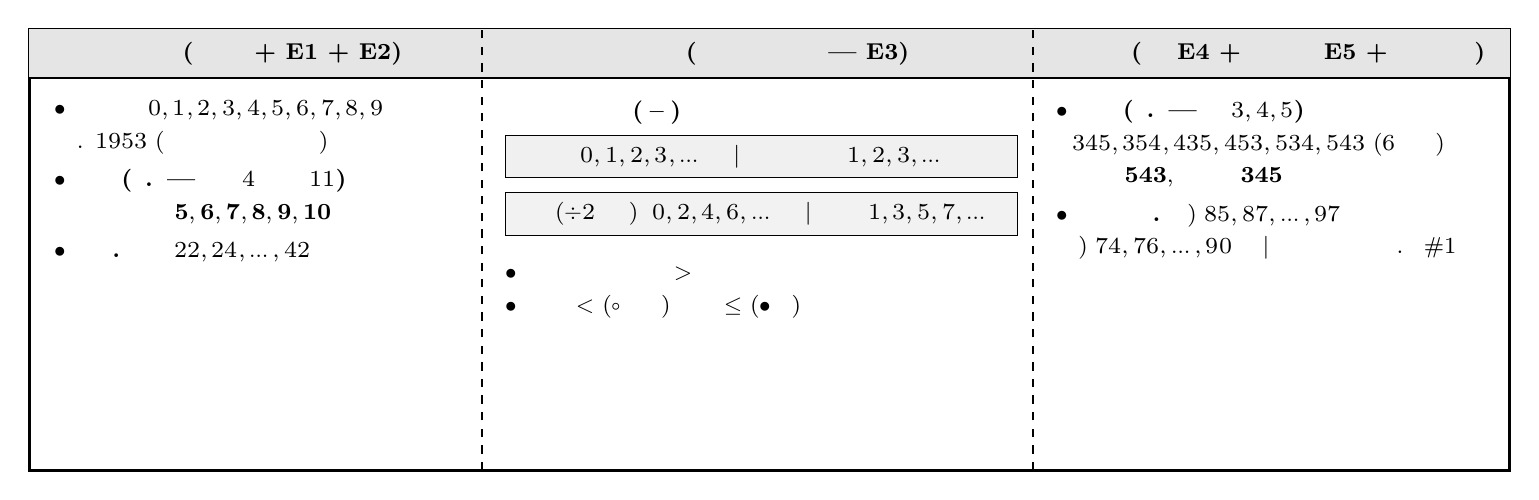
\begin{tikzpicture}[x=1cm, y=1cm, every node/.style={font=\fontsize{8.3pt}{11.8pt}\selectfont, text=black}]
  \draw[black, line width=1.1pt] (0,0) rectangle (18.8,5.60);
  \fill[gray!20] (0,4.98) rectangle (18.8,5.60);
  \draw[black, line width=0.7pt] (0,4.98) -- (18.8,4.98);
  \draw[black, dashed, line width=0.7pt] (5.75,0) -- (5.75,5.60);
  \draw[black, dashed, line width=0.7pt] (12.75,0) -- (12.75,5.60);

  \node at (2.875,5.29) {\textbf{ផ្នែកឆ្វេង (មូលដ្ឋាន + \en{E1} + \en{E2})}};
  \node at (9.25,5.29) {\textbf{ផ្នែកកណ្ដាល (ខ្លឹមសារគោលរក្សាទុក — \en{E3})}};
  \node at (15.775,5.29) {\textbf{ផ្នែកស្ដាំ (គំរូ \en{E4} + ប្រតិបត្តិ \en{E5} + កិច្ចការផ្ទះ)}};

  % Left
  \node[anchor=north west, text width=5.35cm] at (0.20,4.82) {%
    $\bullet$ \textbf{លេខ ១០ តួ៖} $0,1,2,3,4,5,6,7,8,9$\\
    \hspace*{0.2cm}ឧ. $1953$ (មួយពាន់ប្រាំបួនរយហាសិបបី)\\[2pt]
    $\bullet$ \textbf{គំរូ ១ (ទំ.២ — ធំជាង $4$ តូចជាង $11$)៖}\\
    \hspace*{0.2cm}លើបន្ទាត់ចំនួន៖ $\mathbf{5, 6, 7, 8, 9, 10}$\\[2pt]
    $\bullet$ \textbf{គំរូទំ.៣៖} គូពី $22, 24, \dots, 42$
  };

  % Center
  \node[anchor=north west, text width=6.65cm] at (5.92,4.82) {%
    {\muol\fontsize{8.5pt}{12pt}\selectfont មេរៀនទី១៖ ចំនួនគត់ \enbf{(}១\enbf{--}៣\enbf{)}}\\[3pt]
    \tikz\node[draw=black, fill=gray!12, inner sep=3.5pt, text width=6.25cm]{%
      ចំនួនគត់៖ $0, 1, 2, 3, \dots$ \quad|\quad គត់ធម្មជាតិ៖ $1, 2, 3, \dots$
    };\\[4pt]
    \tikz\node[draw=black, fill=gray!10, inner sep=3.5pt, text width=6.25cm]{%
      គត់គូ ($\div 2$ ដាច់)៖ $0, 2, 4, 6, \dots$ \quad|\quad សេស៖ $1, 3, 5, 7, \dots$
    };\\[4pt]
    $\bullet$ \textbf{បន្ទាត់ចំនួន៖} ខាងស្ដាំ $>$ ខាងឆ្វេង\\
    $\bullet$ \textbf{ចុងដែន៖} $<$ ($\circ$ មិនយក) ធៀបនឹង $\le$ ($\bullet$ យក)
  };

  % Right
  \node[anchor=north west, text width=5.65cm] at (12.92,4.82) {%
    $\bullet$ \textbf{គំរូ ២ (ទំ.២ — លេខ $3, 4, 5$)៖}\\
    \hspace*{0.2cm}$345, 354, 435, 453, 534, 543$ ($6$ ចំនួន)\\
    \hspace*{0.2cm}ធំបំផុត $\mathbf{543}$, តូចបំផុត $\mathbf{345}$\\[2pt]
    $\bullet$ \textbf{ប្រតិបត្តិទំ.៣៖} ក) $85, 87, \dots, 97$\\
    \hspace*{0.2cm}ខ) $74, 76, \dots, 90$ \quad|\quad \textbf{កិច្ចការផ្ទះ៖} ទំ.១៤ \#1
  };
\end{tikzpicture}
\end{center}

\vfill
\secstrip{២. ចម្លើយផ្ទៀងផ្ទាត់រហ័សសម្រាប់សន្លឹកកិច្ចការសិស្ស \enbf{(}ទំព័រ ១ និង ទំព័រ ២\enbf{)}}{\en{Answer Key}}

\begin{tcolorbox}[
  enhanced, sharp corners, colback=white, colframe=black,
  boxrule=0.8pt, boxsep=2.5pt, top=4.5pt, bottom=4.5pt, left=6pt, right=6pt
]
  \fontsize{9.0pt}{13.6pt}\selectfont
  $\bullet$ \textbf{ផ្នែក \en{E1}៖} \textbf{សិស្ស ខ} ត្រឹមត្រូវ ព្រោះ $0 \div 2 = 0$ (គូ តែមិនមែនធម្មជាតិ) ហើយ $72 < n$ មានន័យថា $n$ ធំជាង $72$ ដាច់ខាត ។\\[2.5pt]
  $\bullet$ \textbf{ផ្នែក \en{E2}៖} \textbf{សកម្មភាព ១៖} $1953$; ចំនួនគត់ / ចំនួនគត់ធម្មជាតិ; ធំបន្ទាប់គឺ $11$ និង $1000$; គំរូ ១៖ $5, 6, 7, 8, 9, 10$ ។ \textbf{សកម្មភាព ២៖} ចែកដាច់នឹង $2$; គូនៅចន្លោះ $20$ និង $43$៖ $22, 24, 26, 28, 30, 32, 34, 36, 38, 40, 42$ ។\\[2.5pt]
  $\bullet$ \textbf{ផ្នែក \en{E4}៖} $354, \ 453, \ 543 \implies 6$ ចំនួន; ធំបំផុត $543$, តូចបំផុត $345$; \en{EIA} (លេខ $0, 4, 5$)៖ តូចបំផុតគឺ $405$ ។\\[2.5pt]
  $\bullet$ \textbf{ផ្នែក \en{E5}៖} \textbf{១) ប្រតិបត្តិ៖} ទំ.២៖ $9, 10, 11, 12, 13, 14, 15, 16, 17, 18$; ទំ.៣ ក៖ $85, 87, 89, 91, 93, 95, 97$; ទំ.៣ ខ៖ $74, 76, 78, 80, 82, 84, 86, 88, 90$ ។ \textbf{២) បិទ \en{E1}៖} សិស្ស ខ ($74$ ដល់ $90$) ។ \textbf{៣) វិនិច្ឆ័យ \en{A--D}៖} \textbf{ជម្រើស \en{C}} ។ \textbf{៤) សំបុត្រចេញ៖} $0$, $1$, និង $534$ ។
\end{tcolorbox}

\vfill
\secstrip{៣. ចម្លើយលម្អិតនៃកិច្ចការផ្ទះ \enbf{(}សៀវភៅគោល ទំ.១៤ លេខ ១ ក និង ខ\enbf{)}}{សៀវភៅគោល ទំ.១៤}

\begin{tcolorbox}[
  enhanced, sharp corners, colback=white, colframe=black,
  boxrule=0.8pt, boxsep=2.5pt, top=4.5pt, bottom=4.5pt, left=6pt, right=6pt
]
  \fontsize{8.9pt}{13.4pt}\selectfont
  $\bullet$ \textbf{លេខ ១ ក (ទំ.១៤ — រកចំនួនគត់ $n$ ដែល $43 < n < 67$)៖} ដោយសញ្ញាទាំងសងខាងជា $<$ (មិនយក $43$ និងមិនយក $67$) គេបានចំនួនគត់ $n$ ទាំង $23$ ចំនួនគឺ៖ $\mathbf{44, 45, 46, 47, 48, 49, 50, 51, 52, 53, 54, 55, 56, 57, 58, 59, 60, 61, 62, 63, 64, 65, 66}$ ។\\[3pt]
  $\bullet$ \textbf{លេខ ១ ខ (ទំ.១៤ — រកចំនួនគត់សេស $a$ ដែល $55 \le a < 65$)៖} ដោយសញ្ញាខាងឆ្វេងជា $\le$ (យក $55$ ព្រោះ $55$ ជាចំនួនសេស) និងខាងស្ដាំជា $<$ (មិនយក $65$) គេបានចំនួនគត់សេស $a$ ទាំង $5$ ចំនួនគឺ៖ $\mathbf{55, 57, 59, 61, 63}$ ។
\end{tcolorbox}

\vfill
\secstrip{៤. ចំណុចប្រុងប្រយ័ត្នគរុកោសល្យសម្រាប់គ្រូ \enbf{(}ការយល់ច្រឡំសំខាន់ៗ និងវិធីកែតម្រូវភ្លាមៗ\enbf{)}}{\en{Pedagogical Watchlist}}

\begin{tcolorbox}[
  enhanced, sharp corners, colback=panelgray, colframe=black,
  boxrule=0.85pt, boxsep=2.5pt, top=4.5pt, bottom=4.5pt, left=6pt, right=6pt
]
  \fontsize{8.8pt}{13.2pt}\selectfont
  $\bullet$ \textbf{អន្ទាក់ទី ១ (ស្ថានភាពនៃលេខ $0$ — \en{Levenson et al., 2007})៖} សិស្សច្រើនច្រឡំថា «$0$ ជាចំនួនគត់ធម្មជាតិ» ឬ «$0$ មិនគូមិនសេស» ។ ចូរសង្កត់ធ្ងន់ថា $0 \div 2 = 0$ (គ្មានសំណល់) ដូច្នេះ $\mathbf{0}$ \textbf{ជាចំនួនគត់គូ} ប៉ុន្តែមិនរាប់ចូលក្នុងចំនួនគត់ធម្មជាតិ ($1, 2, 3, \dots$) ឡើយ ។\\[2.5pt]
  $\bullet$ \textbf{អន្ទាក់ទី ២ (ចុងដែន $<$ ទល់នឹង $\le$ — \en{Akdeniz et al., 2022})៖} ពេលជួប $72 < n \le 90$ ឬ $55 \le a < 65$ ចូរឱ្យសិស្សគូសសញ្ញា $\circ$ លើចុងដែន $<$ (មិនយក) និងសញ្ញា $\bullet$ លើចុងដែន $\le$ (យកប្រសិនបើត្រូវលក្ខខណ្ឌគូ/សេស) មុននឹងសរសេរបញ្ជីចម្លើយ ។
\end{tcolorbox}

\end{document}
